\section*{Introduction}
This homework centers around the predator-prey dynamic, which is one of the most fundamental ecological interaction model in nature.
This report presents the implementation of a two-dimensional particle-based simulation modelling the interaction between rabbits (prey) and wolves (predator) in a habitat with periodic boundary conditions.
The simulation uses a agent based approach, where the agents follow a stochastic movement patterns and interact according to probabilistic rules for reproduction and predation.

\subsection*{Default Simulation Setup}
The baseline simulation uses the following configuration:
\begin{itemize}
\item \textbf{Domain}: A square habitat of size $L = 10$ with periodic boundary conditions.
\item \textbf{Initial populations}: 900 rabbits and 100 wolves distributed uniform randomly across the domain.
\item \textbf{Movement}: Both species move with a Gaussian step size distribution with standard deviation $\sigma = 0.5$.
\item \textbf{Predation}: Wolves can eat each rabbit within a radius of 0.5 with probability 0.02 per time step.
\item \textbf{Reproduction}: Rabbits reproduce with probability 0.02 per time step.
\item \textbf{Mortality}: Rabbits die after reaching a maximum age of $t_d^r = 100$.
\item \textbf{Starvation}: Wolves die after 50 time steps without eating.
\item \textbf{Spatial indexing}: The domain is divided into $20 \times 20$ grid cells, 
\end{itemize}
Further information regarding the implementation can be found in the README.md file in the root folder of the project.

\section{Scenario A: Standard Case}
In Figure~\ref{fig:ex01} we can observe the population dynamics between wolves and rabbits with parameter $\sigma = 0.5$ and $t_d^r = 100$ the system has the for predator prey models typical oscillatory behavior characteristic. For roughly the first 2500 time steps, the simulation has relatively stable oscillations with the rabbits fluctuating between approximately 300 to 1000 individuals, while the wolves population fluctuates roughly around 100. Furthermore you can observe that oscillation of the wolves is slightly delayed (phase difference). This behavior is consistent with the Lotka-Volterra differential equations, which are given as follows:
\begin{equation}
	\begin{aligned}
		 & \frac{d r}{d t}=\alpha r-\beta r w   \\
		 & \frac{d w}{d t}=-\gamma w+\delta r w
	\end{aligned}
	\label{eq:lv}
\end{equation}
where $r$ represents the number of rabbits, $w$ the number of wolves, $\alpha$ the rabbits growth rate, $\beta$ effect of the presence of wolves, $\gamma$ describes the predators death rate and $\delta$ the effect of rabbits present on the growth rate of the wolves.
However after time step 2500 the systems exhibits a more unstable state, showing significantly larger amplitudes. The population of rabbits has two major peaks one with roughly 2500 individuals and another with even more individuals (9000). These peaks are followed by a very steep decrease, similar to a crash. The wolves show a similar peak slightly delayed as reaction to the massive surge in rabbits.\newline
\newline
We can observe several key similarities with Lotka-Volterra equations
\begin{itemize}
	\item Cyclical nature of population changes
	\item Phase lag between predator and prey
	\item Dependency of predator growth on prey availability
\end{itemize}
However, the agent-based model reveals more complex dynamics than the standard Lotka-Volterra model:
\begin{itemize}
	\item Non-uniform oscillations, amplitudes and phases
	\item Extreme population events
	\item Effects of spatial heterogeneity
		\begin{itemize}
			\item Rabbits and Wolves can form clusters, therefore creating "hotspots", where interactions are more frequent. On the other hand there could also be "save zones", where rabbits can multiply rapidly without being eaten.
			\item The agents have finite movement speeds and a wolf can only eat rabbits that are physically close.
			\item Stochastic encounters, the interactions and the chance of meeting depends on probabilistic dynamics.
		\end{itemize}
\end{itemize}
\begin{figure}[H]
	\centering
	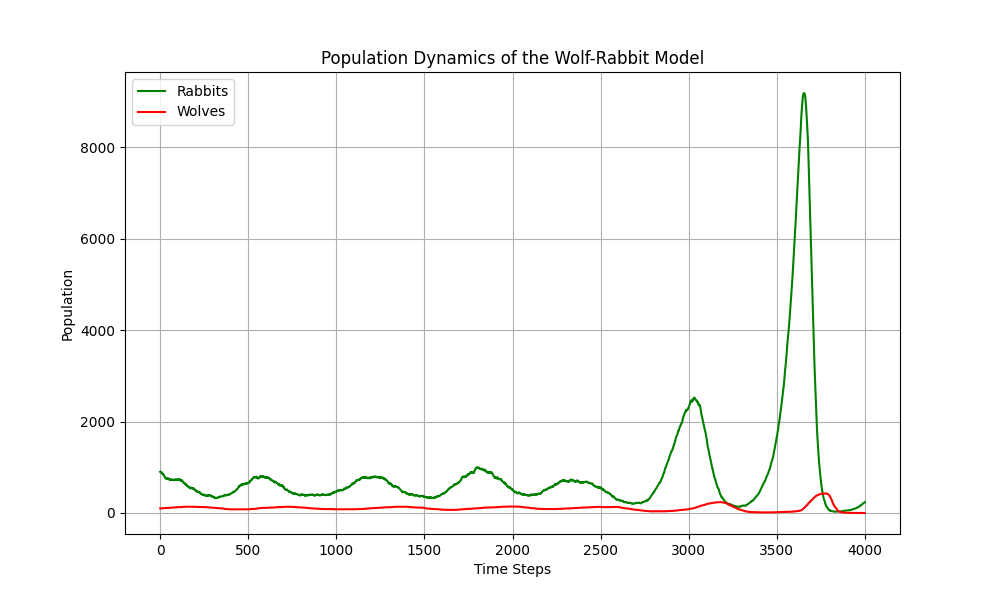
\includegraphics[width=\textwidth]{media/population_dynamics_ex01.png}
	\caption{
		\textbf{Population Dynamics}
		$\sigma = 0.5$, $t_d^r = 100$
	}
	\label{fig:ex01}
\end{figure}

